\chapter{Introduction: Poisson equation in one dimension}
\label{ch:pos1d}

\disclaimer

\section{Introduction}
In this lecture, we provide a brief overview of the variational formulation and the associated finite element approximation using a concrete example: the one-dimensional Poisson equation. The goal is to provide an accessible overview that illustrates the main ideas without complexities associated with higher dimensions and more general equations; we also defer some of the technical discussions to later lectures.

\section{Model problem: strong form}
\label{sec:pos1d_strong}
We consider a taut string with fixed ends subjected to a distributed transverse load as shown in Figure~\ref{fig:pos1d_string}.  Given an appropriate normalization, the shape of the string can be modeled as the solution to a one-dimensional Poisson equation on $\Omega \equiv (0,1)$: %find $u$ such that
\begin{align}
  - \dd{^2u}{x^2} &= f \qquad \text{in } \Omega,  \label{eq:pos1d_strong} \\
  u(x=0) &= 0 \notag , \\
  u(x=1) &= 0 \notag ,
\end{align}
where $f$ is associated with the transverse load.  For an integrable $f$, we may integrate the ODE twice to confirm the existence and uniqueness of the solution.  We refer to this particular form of the problem as the \emph{strong form}.  The name derives from the fact the equation is enforced strongly in the point-wise sense for each $x$ in $\Omega$, which can be contrasted with the \emph{weak form} introduced in the next section. %the nomenclature should become clearer once we introduce the \emph{weak form} in the next section.

\begin{figure}
  \centering
  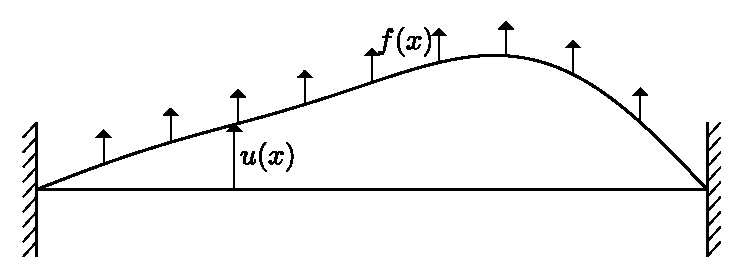
\includegraphics[width=0.6\textwidth]{poisson_string}
  \caption{Taut-string problem modeled by the Poisson equation. \label{fig:pos1d_string}}
\end{figure}

%% One concrete application of the model equation is an elastic bar with fixed ends subjected to distributed force.  The bar is then modeled as
%% \begin{align*}
%%   \sigma &= EA \dd{u}{x} \quad &\text{(Hooke's law)} \\
%%   \dd{\sigma}{x} &= f \quad &\text{(force equilibrium)} \\
%%   u(x=0) = u(x=1) &=0 \quad &\text{(fixed ends)};
%% \end{align*}
%% here $u$ is the displacement, $\sigma$ is the internal force (i.e. area weighted stress), $E$ is the Young's modulus, $A$ is the cross sectional area, and $f$ is the distributed external force. We recognize that the problem fits in the model equation~\eqref{eq:pos1d_strong}.

\section{Variational formulation (or weak formulation)}
\label{sec:pos1d_var}
We now consider a different form of the Poisson equation~\eqref{eq:pos1d_strong} that is (i) more general than the strong form and (ii) amenable to finite element discretization. To obtain this new form of~\eqref{eq:pos1d_strong}, we use the \emph{weighted residual method}. To begin, we choose a (sufficiently regular) test function such that $v(x=0) = v(x=1) = 0$, multiply~\eqref{eq:pos1d_strong} by this function, and integrate the expression to obtain
\begin{equation}
  \int_\Omega v \left( -\dd{^2u}{x^2} \right) dx = \int_\Omega v f dx.
  \label{eq:pos1d_weak_pre}
\end{equation}
We then integrate the left hand side by parts to obtain
\begin{equation}
  \int_\Omega \dd{v}{x} \dd{u}{x} dx - \cancel{ \left[ v \dd{u}{x} \right]_{x=0}^1} = \int_\Omega v f dx;
  \label{eq:pos1d_weak}
\end{equation}
note that the boundary terms vanish because we require $v(x=0) = v(x=1) = 0$. If $u$ is the solution to~\eqref{eq:pos1d_strong}, then we expect the expression~\eqref{eq:pos1d_weak_pre}, and in turn~\eqref{eq:pos1d_weak}, to hold for \emph{any} test function $v$.  In fact, the \emph{variational problem} seeks the solution $u$ which satisfies~\eqref{eq:pos1d_weak} for all suitable test functions $v$.  We may speculate that, given a suitably large set of test functions, the solution $u$ is unique and coincides with the solution to the strong form of the Poisson equation~\eqref{eq:pos1d_strong}.  

We now formalize the above procedure. To this end, we first introduce a linear space
\begin{equation}
  \calV \equiv \{ v \ | \
   v \text{ is continuous, } 
   \int_\Omega \left(\dd{v}{x}\right)^2 dx \text{ is bounded, and } % \text{ is piecewise continuous and bounded on $\Omega$, and } \\
   v(x=0) = v(x=1) = 0 \};
  \label{eq:pos1d_V}
\end{equation}
here, first two conditions are related to the smoothness of the solution sought, and the last condition imposes the boundary conditions. We then define a \emph{bilinear form} $a: \calV \times \calV \to \RR$,
\begin{equation}
  a(w,v) \equiv \int_{\Omega} \dd{v}{x} \dd{w}{x} dx \quad \forall w, v \in \calV,
  \label{eq:pos1d_a}
\end{equation}
and a \emph{linear form} $\ell: \calV \to \RR$,
\begin{equation}
  \ell(v) \equiv \int_{\Omega} v f dx \quad \forall v \in \calV.
  \label{eq:pos1d_ell}
\end{equation}
The form $\ell: \calV \to \RR$ is called a \emph{linear form} because it is linear in the argument in the sense that
\begin{equation*}
  \ell(\alpha w + \beta v) = \alpha \ell(w) + \beta \ell(v) \quad \forall w,v \in \calV, \ \forall \alpha, \beta \in \RR.
\end{equation*}
The form $a: \calV \times \calV \to \RR$ is called a \emph{bilinear form} because 
\begin{align*}
  a(w, \tilde v) & \text{ is a linear form in $w$ for a fixed $\tilde v$, and} \\
  a(\tilde w, v) & \text{ is a linear form in $v$ for a fixed $\tilde w$}.
\end{align*}
Our \emph{variational formulation} of the problem is as follows: find $u \in \calV$ such that
\begin{equation}
  a(u,v) = \ell(v) \quad \forall v \in \calV.
  \label{eq:pos1d_var}
\end{equation}
This variational form of the problem is also called the \emph{weak formulation}.  The space $\calV$ to which the solution $u$ belongs is called the \emph{trial space}; the space $\calV$ to which the test function $v$ belongs is called the \emph{test space}. (While we choose the same trial and test spaces in this example, the two spaces need not be the same in general.)  A variational form which uses the same function space for the trial and test spaces is called the \emph{Galerkin formulation}; our variational form~\eqref{eq:pos1d_var} is a Galerkin formulation because both the trial and test spaces are $\calV$ defined by~\eqref{eq:pos1d_V}. The variational problem has a unique solution; we will study the well-posedness of the problem in subsequent lectures.

We can readily show that the solution to the strong from~\eqref{eq:pos1d_strong} solves the variational form~\eqref{eq:pos1d_var}.  To see this, we integrate by parts and observe that, for all $v \in \calV$,
\begin{equation*}
  a(u,v) - \ell(v) \equiv
  \int_{\Omega} \dd{v}{x} \dd{u}{x} dx - \int_\Omega vf dx
  =
  \int_\Omega v  \underbrace{ \left( -\dd{^2u}{x^2} - f \right) }_{= 0 \text{ as $u$ solves \eqref{eq:pos1d_strong}}}  dx  = 0 ;
\end{equation*}
the boundary terms again vanish because $v(x=0) = v(x=1) = 0$ for all $v \in \calV$. Hence, the solution to the strong form~\eqref{eq:pos1d_strong} satisfies the weak form~\eqref{eq:pos1d_var}, while the converse is not necessarily true.  In fact, the variational form admits more general loads $f$ and associated solutions than the strong form.  For instance, a Dirac delta function, which corresponds to a point load, is an admissible load for the variational formulation \eqref{eq:pos1d_var} and there exists a unique solution to the problem; however, the strong from~\eqref{eq:pos1d_strong} is not well defined for a Dirac delta function $f$ because $f$ does not have well-defined point-wise values. 

\section{Minimization formulation}
\label{sec:pos1d_min}
We now introduce a \emph{minimization form}, which is closely related to the variational form~\eqref{eq:pos1d_var}. We note that not all boundary value problems possess a minimization form; only those problems with an intrinsic energy, such as our model problem~\eqref{eq:pos1d_strong}, possess a minimization form. To obtain a minimization form, we introduce a functional $J: \calV \to \RR$ given by
\begin{equation}
  J(w) \equiv \frac{1}{2} \int_\Omega \left( \dd{w}{x} \right)^2 dx - \int_\Omega f w dx \quad \forall w \in \calV,
  \label{eq:pos1d_J}
\end{equation}
where $\calV$ is defined by~\eqref{eq:pos1d_V}. Our \emph{minimization formulation} is as follows: find $u \in \calV$ such that
\begin{equation}
  u = \argmin_{w \in \calV} J(w).
  \label{eq:pos1d_min}
\end{equation}
For a physical system with intrinsic energy, such as the taut-string problem in Section~\ref{eq:pos1d_strong}, the functional $J$ represents the total energy in the system; $\int_\Omega (\pp{w}{x})^2 dx$ is the internal energy and $\int_\Omega f w dx$ is the external work.  Our minimization statement is hence a statement of energy minimization at the equilibrium. 

%% We can readily show that the solution to the strong form~\eqref{eq:pos1d_strong} solves the minimization problem~\eqref{eq:pos1d_min}.  To see this, let $w = u + v$, where $u \in \calV$ is the solution to~\eqref{eq:pos1d_strong} and $v$ is an arbitrary function in $\calV$.  We then note that $J(w) = J(u+v)$ can be decomposed into three terms:
%% \begin{align*}
%%   J(u+v) &= \frac{1}{2} \int_{\Omega} \left( \dd{(u+v)}{x} \right)^2 dx - \int_\Omega f(u+v) dx \\
%%   &= \underbrace{ \frac{1}{2} \int_{\Omega} \left( \dd{u}{x} \right)^2 dx - \int_\Omega f u dx }_{J(u)}
%%   + \underbrace{ \int_{\Omega} \dd{v}{x} \dd{u}{x} dx - \int_\Omega f v dx }_{J'(u;v) \text{ --- first variation}}
%%   + \underbrace{ \frac{1}{2} \int_{\Omega} \left( \dd{v}{x} \right)^2 dx }_{> 0 \text{ for } v \neq 0}.
%% \end{align*}
%% Here, $J'(u;v)$ denotes the first variation of $J$ at $u$ in the direction $v$.  We integrate by parts $J'(u;v)$ to obtain
%% \begin{align*}
%%   J'(u;v) &= \int_{\Omega} \dd{v}{x} \dd{u}{x} dx - \int_\Omega f v dx
%%   =
%%   - \int_{\Omega} v ( \underbrace{ \dd{^2u}{x^2} + f}_{= 0 \text{ as $u$ solves \eqref{eq:pos1d_strong}}} ) dx + \underbrace{ \left[ v \dd{u}{x} \right]_{x=0}^1 }_{= 0 \text{ as $v$ is in $\calV$}}
%%   = 0;
%% \end{align*}
%% in other words, if $u$ is the solution to the strong form~\eqref{eq:pos1d_strong}, then $J'(u;v) = 0$ for all $v \in \calV$. It thus follows
%% \begin{align*}
%%   J(u + v) = J(u) + \frac{1}{2} \int_\Omega \left( \dd{v}{x} \right)^2 dx
%%   > J(u)  \quad \forall v \neq 0.
%% \end{align*}
%% The solution $u$ to the strong form~\eqref{eq:pos1d_strong} is the minimizer of the functional~\eqref{eq:pos1d_J} and hence the solution to the minimization form~\eqref{eq:pos1d_min}.

%% \section{Variational form}
%% We now consider a \emph{variational form} of the model problem~\eqref{eq:pos1d_strong}. As in the minimization form, we work with the function space~$\calV$ defined in~\eqref{eq:pos1d_V}.

We can readily show that $u \in \calV$ is the solution to the variational problem~\eqref{eq:pos1d_var} if and only if it is the solution to the minimization problem~\eqref{eq:pos1d_min}.  Suppose that $u \in \calV$ is the solution to the variational problem~\eqref{eq:pos1d_var}.  Then, for $w = u + v$ for any $v \in \calV$, we obtain
\begin{align*}
   J(w) = J(u + v) = J(u) + \underbrace{ \int_{\Omega} \dd{v}{x} \dd{u}{x} dx - \int_\Omega f v dx}_{\text{(I)}}
  + \underbrace{ \frac{1}{2} \int_{\Omega} \left( \dd{v}{x} \right)^2 dx }_{\text{(II)}}. %> J(u) \quad \forall v \neq 0.
%  J(w) = J(u + v) = J(u) + \underbrace{ \int_{\Omega} \dd{v}{x} \dd{u}{x} dx - \int_\Omega f v dx}_{= a(u,v) - \ell(v) = 0 \ \forall v \in \calV \text{ by \eqref{eq:pos1d_var}}}
%  + \underbrace{ \frac{1}{2} \int_{\Omega} \left( \dd{v}{x} \right)^2 dx }_{> 0 \text{ for } v \neq 0} > J(u) \quad \forall v \neq 0.
\end{align*}
The term $\text{(I)}$ vanishes because by~\eqref{eq:pos1d_var}
\begin{equation*}
  \int_{\Omega} \dd{v}{x} \dd{u}{x} dx - \int_\Omega f v dx
  = a(u,v) - \ell(v) = 0 \quad \forall v \in \calV.
\end{equation*}
We now analyze $\text{(II)}$.  We first note that the term is greater than $0$ for all non-constant function (i.e. $\dd{v}{x} \neq 0$); $\text{(II)}$ is zero only if $v$ is a constant function.  We next note that for a constant function to satisfy the boundary conditions of $\calV$,  $v(x=0) = v(x=1) = 0$, the function must be the zero function: $ v= 0$. Hence, we conclude that $\text{(II)}$ is greater than $0$ for any non-zero function.  It thus follows that
\begin{equation*}
  J(w) = J(u+v)  > J(u) \quad \forall v \neq 0;
\end{equation*}
hence the solution $u \in \calV$ of the variational problem~\eqref{eq:pos1d_var} solves the minimization problem~\eqref{eq:pos1d_min}. 
Conversely, suppose $u \in \calV$ is the solution to the minimization problem~\eqref{eq:pos1d_min}.  Then, we know that $u$ must be a stationary point of $J$: i.e., $J'(u;v) = 0$, $\forall v \in \calV$; we hence require
\begin{equation*}
  J'(u;v) \equiv
  \int_{\Omega} \dd{v}{x} \dd{u}{x} dx
  - \int_{\Omega} f v dx
  = a(u,v) - \ell(v) = 0 \quad \forall v \in \calV,
\end{equation*}
which is the exact formulation of our variational problem~\eqref{eq:pos1d_var}. Hence we conclude that $u \in \calV$ is the solution to the variational problem~\eqref{eq:pos1d_var} if and only if it is the solution to the minimization problem~\eqref{eq:pos1d_min}; the two problem are equivalent.  It follows that, as noted in  Section~\ref{sec:pos1d_var}, if the solution $u$ solves the strong form~\eqref{eq:pos1d_strong}, then it also the solution to the minimization form~\eqref{eq:pos1d_min}; however, the minimization form admits more general loads $f$ and associated solutions than the strong form. We will soon see that we can derive a finite element approximation from either~\eqref{eq:pos1d_var} or \eqref{eq:pos1d_min}.

\section{Finite element (FE) approximation}
In order to construct a finite element (FE) approximation, we must first choose a suitable subspace of $\calV$ that well approximates $\calV$ and is amenable to computer implementation. To this end, we first \emph{triangulate} the domain $\Omega \equiv (0,1)$ into $N+1$ non-overlapping segments; we introduce points
\begin{equation*}
  0 \equiv x_0 < x_1 < \cdots < x_N < x_{N+1} \equiv 1
\end{equation*}
and segments
\begin{equation*}
  K_i \equiv (x_{i-1}, x_i) \quad i = 1,\dots,N+1.
\end{equation*}
We denote the \emph{triangulation} of the domain $\Omega$, which comprises collection of line segments, by
\begin{equation}
  \calT_h \equiv \{ K_i \}_{i=1}^{N+1}.
  \label{eq:pos1d_Th}
\end{equation}
We denote the length of each segment by $h_i \equiv x_i - x_{i-1}$, $i = 1,\dots,N+1$; a triangulation $\calT_h$ is characterized by the maximum segment length $h \equiv \max_{i=\{ 1,\dots,N+1\}} h_i$.

We now introduce a space of piecewise linear functions defined over our triangulation $\calT_h$ such that they also belong to $\calV$:
\begin{equation}
  \calV_h \equiv \{ v \in \calV \ | \ v|_{K_i} \in \PP^1(K_i), \ i = 1,\dots,N+1\}.
  \label{eq:pos1d_Vh}
\end{equation}
We make a few observations about this particular space.  First, we require that $v$ is in $\calV$ defined by~\eqref{eq:pos1d_V}: (i) $v$ must be continuous, (ii) $\dd{v}{x}$ must be piecewise continuous and bounded, and (iii) $v$ must vanish at the boundaries.  Second, we require $v$ restricted to segment $K_i$ to be in $\PP^1(K_i)$; here, $\PP^1(K_i)$ denotes the space of linear polynomials over $K_i$.  Hence, any function in $\calV_h \subset \calV$ is continuous, piecewise linear, and vanishes at the boundaries. An example of a function in $\calV_h$ is shown in Figure~\ref{fig:pos1d_fe_space}.

\begin{figure}
  \centering
  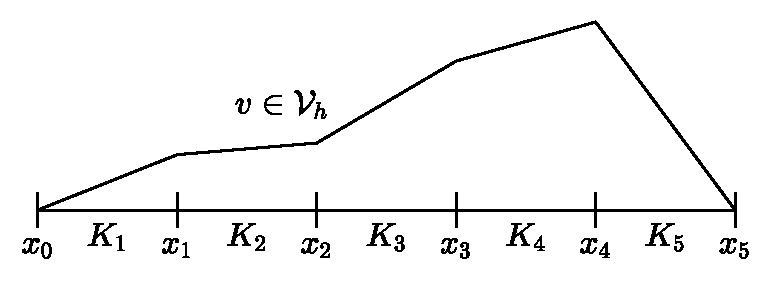
\includegraphics[width=0.6\textwidth]{poisson_fe_space}
  \caption{Linear finite element space for $N = 4$.}
  \label{fig:pos1d_fe_space}
\end{figure}

We can now state our FE approximation problem in either the variational form or the minimization form. The FE variational formulation of our original problem~\eqref{eq:pos1d_var} is as follows: find $u_h \in \calV_h$ such that
\begin{equation}
  a(u_h,v) = \ell(v) \quad \forall v \in \calV_h,
  \label{eq:pos1d_var_fe}
\end{equation}
where $a: \calV \times \calV \to \RR$ and $\ell: \calV \to \RR$ are the bilinear form~\eqref{eq:pos1d_a} and linear form~\eqref{eq:pos1d_ell}, respectively. In words, we seek the solution in and test against the finite-dimensional (hence computable) subspace $\calV_h$ of $\calV$.

Similarly, the FE minimization form is as follows: find $u_h \in \calV_h$ such that
\begin{equation}
  u_h = \argmin_{v \in \calV_h} J(v),
  \label{eq:pos1d_min_fe}
\end{equation}
where $J: \calV \to \RR$ is the energy functional~\eqref{eq:pos1d_J}. In words, we seek the minimizer of $J$ in the subspace $\calV_h$ of $\calV$.  %Note that $v \in \calV_h$ is an admissible argument of $J$ since $\calV_h \subset \calV$.
As before, $u_h \in \calV_h$ is the solution to the FE minimization problem~\eqref{eq:pos1d_min_fe} if and only if it is the solution to the FE variational problem~\eqref{eq:pos1d_var_fe}. We will henceforth refer to $u_h$ as the \emph{finite element solution}.


\section{Finite element approximation: implementation}
We now wish to develop a computationally tractable formulation such that we can implement~\eqref{eq:pos1d_var_fe} (or equivalently~\eqref{eq:pos1d_min_fe}) and find an approximation to the original problem~\eqref{eq:pos1d_var} (or equivalently~\eqref{eq:pos1d_min}).  To this end, we introduce a \emph{basis} for $\calV_h$ defined in~\eqref{eq:pos1d_Vh}.  A convenient basis for $\calV_h$ is a \emph{Lagrange basis}  $\{\phi_i\}_{i=1}^N$ comprised piecewise linear polynomials such that 
\begin{equation*}
  \phi_i(x_j) = \delta_{ij} \equiv  \begin{cases}
    1 \quad j = i \\
    0 \quad j\neq i
  \end{cases},
  \quad j = 0,\dots,N+1;
\end{equation*}
in words, $\phi_i$ is a continuous piecewise linear function that is takes the value of 1 at the interpolation point $x_i$ and the value of 0 at all other interpolation points.  These basis functions are shown in Figure~\ref{fig:pos1d_basis}.

\begin{figure}
  \centering
  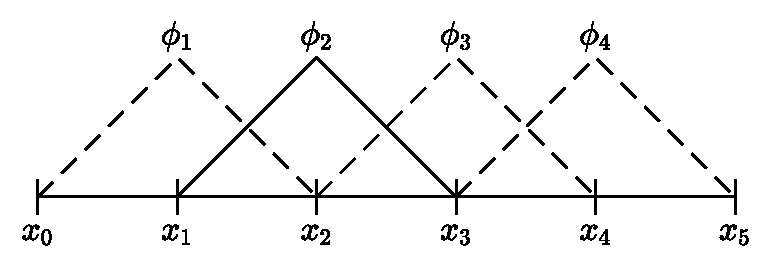
\includegraphics[width=0.6\textwidth]{poisson_1d_basis}
  \caption{Basis functions for a linear finite element space for $N = 4$.}
  \label{fig:pos1d_basis}
\end{figure}

We can show that $\{ \phi_i \}_{i=1}^N$ is indeed a basis for $\calV_h$: the set (i) is linearly independent and (ii) spans $\calV_h$. To show the set is linearly independent, we must show that $\sum_{i=1}^n c_i \phi_i(x) = 0$ implies $c_i = 0$, $i = 1,\dots,N$; the statement holds because, for $\sum_{i=1}^n c_i \phi_i(x) = 0$, we must have $\sum_{i=1}^n c_i \phi_i(x_j) = \sum_{i=1}^n c_i \delta_{ij} = c_j = 0$, $j = 1,\dots,N$. To show the set spans $\calV_h$, we observe that any $v \in \calV_h$ can be expressed as
\begin{equation*}
  v = \sum_{i=1}^N \hat v_i \phi_i
\end{equation*}
for $\hat v_i \equiv v(x_i)$. (The coefficients are also unique because the set is linearly independent.)  We hence conclude that $\{\phi_i\}_{i=1}^N$ is a basis for $\calV_h$. 

%% We can readily show that $\{ \phi_i \}_{i=1}^N$ is indeed a basis for $\calV_h$: i.e., $\calV_h = \text{span}\{ \phi_i \}_{i=1}^N$ and $\{\phi_i\}_{i=1}^N$ is linearly independent. We note that for \emph{any} function $v \in \calV_h$, there exists a \emph{unique} coefficients $\hat v \in \RR^N$ such that 
%% \begin{equation*}
%%   v(x) = \sum_{i=1}^N \hat v_i \phi_i(x), \quad x \in \Omega.
%% \end{equation*}
%% In particular, the choice $\hat v_i = v(x_i)$ yields the desired equality.

We now restate the FE variational problem~\eqref{eq:pos1d_var_fe} using the basis and associated coefficients.  Specifically, we represent $u_h \in \calV_h$ and $v \in \calV_h$ as 
\begin{align}
  u_h &\equiv \sum_{j=1}^N \hat u_{h,j} \phi_j \label{eq:pos1d_uh_rep} \\
   v &\equiv \sum_{i=1}^N \hat v_i \phi_i \notag
\end{align}
for some $\hat u_h \in \RR^N$ and $\hat v \in \RR^N$, and consider the following equivalent problem: find $\hat u_h \in \RR^N$ such that
\begin{equation}
  a(\sum_{j=1}^N \hat u_{h,j} \phi_j, \sum_{i=1}^N \hat v_i \phi_i) - \ell(\sum_{i=1}^N \hat v_i \phi_i)
  =
  \sum_{i=1}^N \sum_{j=1}^N \hat v_i a(\phi_j, \phi_i) \hat u_{h,j} -
  \sum_{i=1}^N \hat v_i \ell(\phi_i) = 0 \quad \forall \hat v \in \RR^N.
  \label{eq:pos1d_fe_disc_step_1}
\end{equation}
Here, we have appealed to the bilinearity and linearity of $a(\cdot,\cdot)$ and $\ell(\cdot)$, respectively. We then note that in~\eqref{eq:pos1d_fe_disc_step_1} we can replace the condition $\forall \hat v \in \RR^N$ with an equivalent condition that the statement holds $\hat v \in \{e_i \}_{i=1}^N$, where $\{e_i\}_{i=1}^N$ is the canonical basis of $\RR^N$ (i.e.~$e_i \in \RR^N$ has $1$ in the $i$-th entry and $0$ elesewhere). Then, we can restate~\eqref{eq:pos1d_fe_disc_step_1} as follows: find $\hat u_h \in \RR^N$ such that
\begin{equation}
  \sum_{j=1}^N a(\phi_j,\phi_i) \hat u_{h,j} = \ell(\phi_i) \quad  \forall i = 1,\dots,N.
  \label{eq:pos1d_sys}
\end{equation}
We can also rewrite the linear system in the matrix form:
\begin{equation*}
  \underbrace{ \bmat{ccc}
  a(\phi_1,\phi_1) & \cdots & a(\phi_N,\phi_1) \\
  \vdots & \ddots & \vdots \\
  a(\phi_1,\phi_N) & \cdots & a(\phi_N,\phi_N) \\
  \emat
  }_{A_h \in \RR^{N \times N}}
  \underbrace{ \bmat{c} \hat u_{h,1}  \\ \vdots \\ \hat u_{h,N} \emat }_{\hat u_h \in \RR^N}
  =
  \underbrace{ \bmat{c} \ell(\phi_1) \\ \vdots \\ \ell(\phi_N) \emat }_{\hat f_h \in \RR^N},
\end{equation*}
or, more concisely,
\begin{equation*}
  A_h \hat u_h = f_h.
\end{equation*}
The matrix $A_h$ is called the \emph{stiffness matrix} and the vector $f_h$ is called the \emph{load vector}.% The linear system is in fact \emph{symmetric positive definite} (SPD) and hence has a unique solution.

%\section{Solution of $A_h \hat u_h = f_h$}

We now take a closer look at the matrix $A_h \in \RR^{N \times N}$ associated with our particular choice of the basis $\{\phi_i\}_{i=1}^N$.  We consider four distinct parts of the matrix: the main diagonal, superdiagonal, subdiagonal, and all other entries.  The diagonal entries are given by 
\begin{equation*}
  a(\phi_i,\phi_i) = \int_{x_{i-1}}^{x_{i+1}} \dd{\phi_i}{x} \dd{\phi_i}{x} dx
  = \int_{x_{i-1}}^{x_{i}} \left( \frac{1}{h_i} \right)^2 dx +
  \int_{x_{i}}^{x_{i+1}} \left( - \frac{1}{h_{i+1}} \right)^2 dx
  = \frac{1}{h_i} + \frac{1}{h_{i+1}}, \quad i = 1,\dots,N.
\end{equation*}
The superdiagonal entries are given by
\begin{equation*}
  a(\phi_i,\phi_{i+1}) =
  \int_{x_i}^{x_{i+1}} \dd{\phi_i}{x} \dd{\phi_{i+1}}{x} dx
  = \int_{x_i}^{x_{i+1}} \left( - \frac{1}{h_i} \right) \left( \frac{1}{h_i} \right) dx
  = - \frac{1}{h_i}, \quad i = 1,\dots,N-1.
\end{equation*}
The subdiagonal entries are given by
\begin{equation*}
  a(\phi_{i+1},\phi_i) =
  \int_{x_i}^{x_{i+1}} \dd{\phi_{i+1}}{x} \dd{\phi_i}{x} dx
  = \int_{x_i}^{x_{i+1}}  \left( \frac{1}{h_i} \right) \left( - \frac{1}{h_i} \right) dx
  = - \frac{1}{h_i}, \quad i = 1,\dots,N-1.
\end{equation*}
All other entries are zero because $\phi_i$ and $\phi_j$ do not overlap for $|i -j| > 1$.

We now consider the simple case of equispaced nodes so that $h_i = h$, $\forall i = 1,\dots,N$.  The associated stiffness matrix is
\begin{equation*}
  A_h = \frac{1}{h} \bmat{ccccc} 2 & -1 \\ -1 & 2 & -1 \\ & \ddots & \ddots & \ddots \\ & &-1 & 2 & -1 \\ &&& -1 & 2 \emat.
\end{equation*}
We observe that the matrix is \emph{sparse} and in particular \emph{tridiagonal}.  Moreover, this matrix is symmetric positive definite.  The symmetry is obvious from inspection; the positive definiteness follows from 
\begin{align*}
  \hat v^T A_h \hat v
  &=
  \frac{1}{h} \left(
  2\sum_{i=1}^N \hat v_i^2 - 2\sum_{i=1}^{N-1} \hat v_i\hat v_{i+1} 
  \right)
  =
  \frac{1}{h} \left(
  \hat v_1^2 + \hat v_{N}^2 + \sum_{i=1}^{N-1} (\hat v_i - \hat v_{i+1})^2 
  \right)
  > 0 \quad \forall \hat v \neq 0.
\end{align*}
Hence the solution exists and is unique.  The storage requirement for the tridiagonal system is $\calO(N)$, and the solution to $A_h \hat u_h = f_h$ can be obtained using the Thomas algorithm, which is a form of Gaussian elimination, in $\calO(N)$ floating point operations.  Given the solution  $\hat u_h \in \RR^N$ to the linear system, our finite element solution $u_h \in \calV_h$ to the FE variational formulation~\eqref{eq:pos1d_var_fe} (or equivalently~\eqref{eq:pos1d_min_fe}) is given by the representation~\eqref{eq:pos1d_uh_rep}.

\section{An error estimate: optimality and polynomial approximation}
We now assess how accurately our finite element solution $u_h \in \calV_h$ to~\eqref{eq:pos1d_var_fe} (or equivalently~\eqref{eq:pos1d_min_fe}) approximates the solution $u \in \calV$ to~\eqref{eq:pos1d_var} (or equivalently~\eqref{eq:pos1d_min}).  To this end, we need to first define a norm with which we can measure the ``closeness'' of the approximation. In particular, we introduce the \emph{energy norm} associated with the model problem,
\begin{equation*}
  \enorm{v} \equiv \sqrt{a(v,v)}  = \left( \int_{\Omega} \left( \dd{v}{x} \right)^2 dx \right)^{1/2} \quad \forall v \in \calV.
\end{equation*}
Because $\enorm{ \cdot }$ is the induced norm associated with an inner product $a(\cdot,\cdot)$ over $\calV$, it is indeed a proper norm that satisfies i) scalability, ii) triangle inequality, and iii) positivity.  

We next state a key ingredient of the FE error estimate: \emph{Galerkin orthogonality}: since $\ell(v) = a(u,v)$, $\forall v \in \calV$, the FE variational statement~\eqref{eq:pos1d_var_fe} implies
\begin{equation*}
  0 = \ell(v) - a(u_h,v) = a(u,v) - a(u_h,v) = a(u-u_h,v) = 0 \quad \forall v \in \calV_h;
\end{equation*}
the relationship is called Galerkin orthogonality because it states that the error $u - u_h$ is orthogonal to the space $\calV_h$ in the inner product $a(\cdot,\cdot)$. We now observe that, for any $w_h \in \calV_h$,
\begin{align*}
  \enorm{u-u_h}^2
  &=
  a(u-u_h, u-w_h) + \underbrace{ a(u-u_h,w_h - u_h) }_{= 0 \text{ by Galerkin orthogonality}}
  \\
  &=
  a(u-u_h, u - w_h)% & \text{(Galerkin orthogonality)}
  \\
  &\leq  \enorm{u - u_h} \enorm{u - w_h}. & \text{(Cauchy-Schwarz inequality)}.
\end{align*}
It follows that
\begin{equation}
  \enorm{u - u_h} \leq \enorm{u - w_h} \quad \forall w_h \in \calV_h,
  \label{eq:pos1d_fe_opt}
\end{equation}
or, equivalently,
\begin{equation*}
  \enorm{u-u_h} = \inf_{w_h \in \calV_h} \enorm{u - w_h}.
\end{equation*}
We observe that the FE approximation $u_h \in \calV_h$ is \emph{optimal} in the energy norm in the sense that it is the closest approximation to the solution $u \in \calV$ out of all elements in $\calV_h$.  In other words, even if we knew the solution $u$, we could not have found a better solution in $\calV_h$ than $u_h$.

As the optimality statement~\eqref{eq:pos1d_fe_opt} holds for any $w_h \in \calV_h$, we can set $w_h = \calI_h u = \sum_{i=1}^N u(x_i) \phi_i$, the polynomial interpolant associated with our Lagrange basis functions.  It can be shown that for any $v \in \calV$ the following interpolation error bounds hold:
\begin{align*}
  \enorm{v - \calI_h v} &\leq \frac{1}{8} h^2 \max_{x \in \Omega} |v''(x)| \\
  \enorm{\dd{v}{x} - \dd{(\calI_h u)}{x}} &\leq h \max_{x \in \Omega} |v''(x)| .
\end{align*}
(We will later derive the bounds in a more formal setting.) We hence arrive at the following FE error bound in terms of the discretization parameter $h$:
\begin{equation*}
  \enorm{u - u_h} \leq \enorm{u - \calI_h u} \leq h \max_{x \in \Omega}  | u''(x) |.
\end{equation*}
In words, the energy-norm error of our finite element solution $u_h \in \calV_h$  depends on  (i)the maximum second derivative over the domain and (ii) the triangulation parameter $h$.

To demonstrate the convergence of the finite element approximation, we consider the Poisson problem~\eqref{eq:pos1d_strong} for $f = 1$. The exact solution is $u(x) = x(1-x)/2$. Figure~\eqref{fig:pos1d_conv} shows that the energy norm of the error $\enorm{u - u_h}$ converges at the rate of $h^1$ as predicted by theory.
\begin{figure}
  \centering
  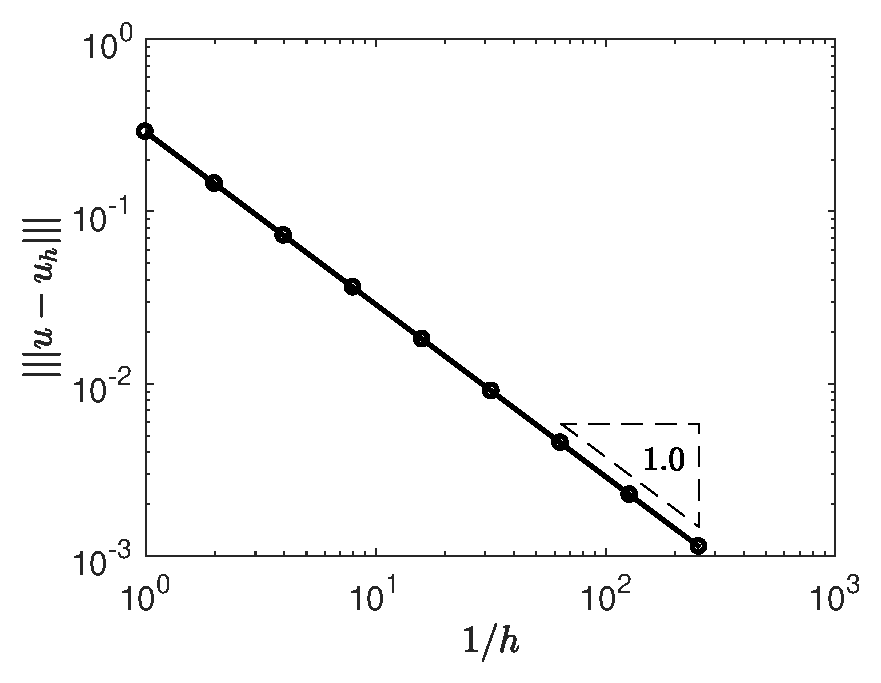
\includegraphics[width=0.5\textwidth]{poisson_1d_conv}
  \caption{Convergence of the finite element approximation for $-\Delta u = 1$.}
  \label{fig:pos1d_conv}
\end{figure}

\section{Summary}
In this lecture, we considered the variational formulation and the associated finite element approximation of the one-dimensional Poisson equation to introduce the main ideas without the complexities associated with higher dimensions and more general equations.  We summarize key points of the lecture:
\begin{enumerate}
\item A one-dimensional Poisson problem can be written in the strong form, minimization form, or variational (or weak) form. 
\item The solution to the strong form is also the solution to the minimization and variational form, but the converse is not true in general.  The minimization and variational forms admit more general loads $f$ and the associated solutions.
\item A finite element approximation space $\calV_h$ is a subspace of $\calV$.  In one dimension, we may choose $\calV_h$ as the space of piecewise linear polynomials associated with a triangulation of $\Omega \subset \RR^1$ into segments.
\item The finite element solution is the solution of the minimization or variational problem in the finite element subspace $\calV_h \subset \calV$.
\item Given a basis for $\calV_h$, the finite element solution can be computed in a systematic manner by assembling the associated stiffness matrix and load vector and then solving the resulting linear system.
\item For the Poisson equation, the finite element approximation $u_h$ is optimal in energy norm; even \emph{if} we knew the exact solution $u \in \calV$, we could not have found a better solution in $\calV_h$ than $u_h$.
\item The error in the linear finite element approximation of the Poisson equation converges as $h^1$ in energy norm, where $h$ is the mesh spacing.
\end{enumerate}
